\documentclass{article}
\usepackage[margin=1in]{geometry}
\usepackage{natbib}
\usepackage{amsmath}
\usepackage{graphicx}
\usepackage{color}
\usepackage[procnames]{listings}
\usepackage{textcomp}
\usepackage{setspace}
\usepackage{palatino}

\usepackage{enumitem}
\usepackage{array}
\setlist{nolistsep}

\usepackage{floatrow}
\usepackage{sidecap}
\sidecaptionvpos{figure}{c}
\usepackage{wrapfig}
\usepackage{float}
\usepackage{framed}
\usepackage{caption}



\definecolor{gray}{gray}{0.2}
\definecolor{green}{rgb}{0,0.5,0}
\definecolor{lightgreen}{rgb}{0,0.7,0}
\definecolor{purple}{RGB}{160,90,180}
\definecolor{darkred}{rgb}{0.6,0,0}
\definecolor{orange}{rgb}{1,0.3,0}
\definecolor{comments}{RGB}{94,148,148}
%\definecolor{comments}{RGB}{102, 153, 153}
\definecolor{medblue}{RGB}{65,105,225}
\definecolor{lightgray}{rgb}{0.98, 0.98, 0.98}
\definecolor{medgray}{rgb}{0.925, 0.925, 0.925}
\definecolor{pink}{rgb}{0.8, 0, 0.8}
\definecolor{orangey}{RGB}{232, 150, 25}


\setlength\parindent{0pt}
\usepackage[T1]{fontenc} % quotes

	
\newcommand{\code}[1]{\texttt{\small{#1}}}

%\newcommand{\code}[1]{\textbf{\texttt{\small{#1}}}}

\usepackage{hyperref}
\hypersetup{
	colorlinks=true, %set true if you want colored links
	linktoc=all,     %set to all if you want both sections and subsections linked
	linkcolor=blue,  %choose some color if you want links to stand out
	urlcolor=blue
}



\lstset{
		language=python,
		rulecolor=\color{black},
		frame=leftline,
		backgroundcolor=\color{medgray},
		numbers=left,
		numberstyle=\scriptsize,
		basicstyle=\ttfamily\small\setstretch{1.2},
		stringstyle=\color{red},
		showstringspaces=false,
		alsoletter={1234567890},
		otherkeywords={\ , \}, \{},
		breaklines=true,
		keywordstyle=\ttfamily,
		emph={access,and,as,break,class,continue,def,del,elif,else,%
			except,exec,finally,for,from,global,if,import,in,is,%
			lambda,not,or,pass,print,raise,return,try,while,assert},
		emphstyle=\color{purple}\bfseries,
		emph={[2]self},
		emphstyle=[2]\color{gray},	
		emph={[4]ArithmeticError,AssertionError,AttributeError,BaseException,%
			DeprecationWarning,EOFError,Ellipsis,EnvironmentError,Exception,%
			False,FloatingPointError,FutureWarning,GeneratorExit,IOError,%
			ImportError,ImportWarning,IndentationError,IndexError,KeyError,%
			KeyboardInterrupt,LookupError,MemoryError,NameError,None,%
			NotImplemented,NotImplementedError,OSError,OverflowError,%
			PendingDeprecationWarning,ReferenceError,RuntimeError,RuntimeWarning,%
			StandardError,StopIteration,SyntaxError,SyntaxWarning,SystemError,%
			SystemExit,TabError,True,TypeError,UnboundLocalError,UnicodeDecodeError,%
			UnicodeEncodeError,UnicodeError,UnicodeTranslateError,UnicodeWarning,%
			UserWarning,ValueError,Warning,ZeroDivisionError,abs,all,any,apply,%
			basestring,bool,buffer,callable,chr,classmethod,cmp,coerce,compile,%
			complex,copyright,credits,delattr,dict,dir,divmod,enumerate,eval,%
			execfile,exit,filter,float,frozenset,getattr,globals,hasattr,%
			hash,help,hex,id,input,int,intern,isinstance,issubclass,iter,len,%
			license,list,locals,long,map,max,min,object,oct,open,ord,pow,property,%
			quit,range,raw_input,reduce,reload,repr,reversed,round,set,setattr,%
			slice,sorted,staticmethod,str,sum,super,tuple,unichr,unicode,%
			vars,xrange,zip},
		emphstyle=[4]\color{purple}\bfseries,
		emph={[5]assign_name,num_classes,codon_model,read_tree,print_tree,%
			branch_het,site_het,compute_frequencies,Site,Evolver,Genetics,%
			MatrixBuilder,aminoAcid_Matrix,nucleotide_Matrix,mechCodon_Matrix,%
			mutSel_Matrix,ECM_Matrix,EvoModels,Model,Tree,Partition,%
			StateFrequencies,EqualFrequencies,RandomFrequencies,CustomFrequencies,%
			ReadFrequencies,EmpiricalModelFrequencies},
		emphstyle=[5]\color{medblue}\bfseries,		
		upquote=true,
		morecomment=[s][\color{comments}]{"""}{"""},
		morecomment=[s][\color{comments}]{'''}{'''},
		commentstyle=\color{comments}\slshape,
		literate={>>>}{\textbf{\textcolor{comments}{>{>}>}}}3,
		procnamekeys={def,class},
		procnamestyle=\color{green}\textbf,
		tabsize=4	
}


% Python for external files
\newcommand\pythonexternal[2][]{{
		\lstinputlisting[#1]{#2}}}

% Python for inline
\newcommand\pythoninline[1]{{\lstinline!#1!}}



\begin{document}


\begin{titlepage}
	\begin{center}
	
		
	\textsc{\Huge Pyvolve User Manual}\\[1cm]
		
	{\huge Stephanie J. Spielman}\\[0.5cm]
	
	{\large Email: stephanie.spielman@gmail.com}

	\vspace*{1.5cm}
	
\includegraphics[width=1.5in]{pyvolve_logo_manual.png}
	
	
	
	\end{center}
	
	
\end{titlepage}

\newpage

\tableofcontents

\newpage


\section{Introduction}

Pyvolve is an open-source Python module for simulating genetic data along a phylogeny using Markov models of sequence evolution, according to standard methods \cite{Yang2006}. Pyvolve is freely available under a FreeBSD license and is hosted on github:
\href{http://sjspielman.org/pyvolve/}{http://sjspielman.org/pyvolve/}. Pyvolve has several dependencies, including \href{http://biopython.org/wiki/Download}{BioPython}, \href{http://www.scipy.org/install.html}{NumPy}, and \href{http://www.scipy.org/install.html}{SciPy}. These modules must be properly installed and in your Python path. Please file any and all bug reports on the github repository \href{https://github.com/sjspielman/pyvolve/issues}{Issues} section.

Pyvolve is written such that it can be seamlessly integrated into your Python pipelines without having to interface with external software platforms. However, please note that for extremely large ($>$1000 taxa) and/or extremely heterogenous simulations (e.g. where each site evolves according to a unique evolutionary model), Pyvolve may be quite slow and thus may take several minutes to run. Faster sequence simulators you may find useful are detailed in ref.\ \citep{Arenas2012}, which gives an overview of various sequence simulation softwares (from 2012).

Pyvolve supports a variety of evolutionary models, including the following:
\begin{itemize}
	\item Nucleotide Models 
	\begin{itemize}
		\item Generalized time-reversible model \cite{GTR} and all nested variants
	\end{itemize}
	\item Amino-acid exchangeability models 
	\begin{itemize}
		\item JTT \cite{JTT}, WAG \cite{WAG}, LG \cite{LG}, mtmam \cite{YangNielsenHasagawa1998}, mtREV24 \cite{mtrev24}, and DAYHOFF \cite{dayhoff}
	\end{itemize}
	\item Codon models
	\begin{itemize}
		\item Mechanistic ($dN/dS$) models (MG-style \cite{MG94} and GY-style \cite{GY94})
		\item Empirical codon model \cite{ECM}
	\end{itemize}
	\item Mutation-selection models
	\begin{itemize}
		\item Halpern-Bruno model \cite{HB98}, implemented for codons and nucleotides
	\end{itemize}
\end{itemize}
\renewcommand{\arraystretch}{1.75} %table row spacing, defined here to avoid affecting title
\setlength{\parskip}{12pt}

Both site- and branch- (temporal) heterogeneity are supported. A detailed and highly-recommended overview of Markov process evolutionary models, for DNA, amino acids, and codons, is available in the book \emph{Computational Molecular Evolution}, by Ziheng Yang \citep{Yang2006}.

Although Pyvolve does not simulate insertions and deletions (indels), Pyvovle does include several novel options not available (to my knowledge) in other sequence simulation softwares. These options, detailed in Section~\ref{sec:special}, include custom rate-matrix specification, novel matrix-scaling approaches, and branch length perturbations.

\section{Installation}

Pyvolve may be downloaded and installed using \code{pip} or \code{easy\_install}. Source code is available from \href{https://github.com/sjspielman/pyvolve/releases}{https://github.com/sjspielman/pyvolve/releases}.

\section{Citation}

If you use Pyvolve, or code derived from Pyvolve, please cite us:

Spielman, SJ and Wilke, CO. 2015. "Pyvolve: A flexible Python module for simulating sequences along phylgenies." biorXiv. doi: \href{http://dx.doi.org/10.1101/020214}{http://dx.doi.org/10.1101/020214}.

\section{Basic Usage}

Similar to other simulation platforms, Pyvolve evolves sequences in groups of \textbf{partitions} (see, for instance, the Indelible simulation platform \citep{Fletcher2009}). Each partition has an associated size and model (or set of models, if branch heterogeneity is desired). Note that all partitions will evolve according to the same phylogeny\footnote{If you wish to have different partitions evolve according to distinct phylogenies, I recommend performing several simulations and then merging the resulting alignments in the post-processing stage.}. 

The general framework for a simple simulation is given below. In order to simulate sequences, you must define the phylogeny along which sequences evolve as well as any evolutionary model(s) you'd like to use, and assign model(s) to partition(s). Each evolutionary model has associated parameters which you can customize, as detailed in Section~\ref{sec:evomodels}.

\begin{lstlisting}
######### General pyvolve framework #########
#############################################

# Import the Pyvolve module
import pyvolve

# Read in phylogeny along which Pyvolve should simulate
my_tree = pyvolve.read_tree(file = "file_with_tree_for_simulating.tre")

# Define evolutionary model(s) with the Model class
my_model = pyvolve.Model(<model_type>, <custom_model_parameters>)

# Define partition(s) with the Partition class
my_partition = pyvolve.Partition(models = my_model, size = 100)

# Evolve partitions with the callable Evolver class
my_evolver = pyvolve.Evolver(tree = my_tree, partitions = my_partition)
my_evolver() # evolve sequences
\end{lstlisting}

Each of these steps is explained below, in detail with several examples. For additional information, consult the API documentation, at \href{http://sjspielman.org/pyvolve}{http://sjspielman.org/pyvolve}. Further, all functions and classes in Pyvolve have highly descriptive docstrings, which can be accessed with Python's \code{help()} function. 


\section{Defining phylogenies}\label{sec:phylogeny}

Phylogenies must be specified as newick strings (see \href{https://en.wikipedia.org/wiki/Newick_format}{this wikipedia page} for details) \emph{with branch lengths}. Pyvolve reads phylogenies using the function \code{read\_tree}, either from a provided file name or directly from a string:
\begin{lstlisting}
# Read phylogeny from file with the keyword argument "file"
phylogeny = pyvolve.read_tree(file = "/path/to/tree/file.tre")

# Read phylogeny from string with the keyword argument "tree"
phylogeny = pyvolve.read_tree(tree = "(t4:0.785,(t3:0.380,(t2:0.806,(t5:0.612,t1:0.660):0.762):0.921):0.207);")
\end{lstlisting}

To implement branch (temporal) heterogeneity, in which different branches on the phylogeny evolve according to different models, you will need to specify \emph{model flags} at particular nodes in the newick tree, as detailed in Section~\ref{sec:branchhet}.

Further, to assess that a phylogeny has been parsed properly (or to determine the automatically-assigned names of internal nodes), use the \code{print\_tree} function:
\begin{lstlisting}
# Read phylogeny from string
phylogeny = pyvolve.read_tree(tree = "(t4:0.785,(t3:0.380,(t2:0.806,(t5:0.612,t1:0.660):0.762):0.921):0.207);")

# Print the parsed phylogeny
pyvolve.print_tree(phylogeny)
## Output from the above statement: node_name  branch_length  model_flag
'''
>>>     t4 0.785 None
>>>     internal_node3 0.207 None
>>>         t3 0.38 None
>>>         internal_node2 0.921 None
>>>              t2 0.806 None
>>>              internal_node1 0.762 None
>>>                  t5 0.612 None
>>>                  t1 0.66 None 
'''
\end{lstlisting}
In the above output, tabs represent nested hierarchies in the phylogeny. Each line shows the node name (either a tip name, "root", or an internal node), the branch length leading to that node, and the model flag associated with that node. This final value will be \code{None} if model flags are not provided in the phylogeny. Again, note that model flags are only required in cases of branch heterogeneity (see Section~\ref{sec:branchhet}).


\section{Defining Evolutionary Models}\label{sec:evomodels}

The evolutionary models built into Pyvolve are outlined in Table 1 of this manual. Pyvolve uses \code{Model} objects to store evolutionary models:
\begin{lstlisting}
# Basic framework for defining a Model object (second argument optional)
my_model = Model(<model_type>, <custom_model_parameters_dictionary>)
\end{lstlisting}
A single argument, \code{$<$model\_type$>$}, is required when defining a \code{Model} object. Available model types are shown in Table 1. Each model type has various associated parameters, which can be customized via the second optional argument to \code{Model}, written above as \code{$<$custom\_model\_parameters\_dictionary$>$}. This argument should be a dictionary of parameters to customize, and each modeling framework has particular keys which can be included in this dictionary. Available model types and associated customizable parameters are shown in Table 1 and detailed in the subsections below. 

Note that there are several additional optional keyword arguments which may be passed to \code{Model}, including arguments pertaining to site-rate heterogeneity (see Section~\ref{sec:sitehet}) and the matrix scaling algorithm (see Section~\ref{sec:scaling}).


\begin{table}[H]
	\centering

	{
		\scalebox{0.8}{
		\begin{tabular}{>{\centering\arraybackslash}p{1.5in} >{\centering\arraybackslash}p{2in} >{\raggedright}p{4in}}
		\hline

		\multicolumn{1}{c}{\textbf{Modeling framework}}  & \multicolumn{1}{c}{\textbf{Pyvolve model type(s)}} & \multicolumn{1}{c}{\textbf{Optional parameters} (\code{"key"})}
		\tabularnewline 
		\hline
		Nucleotide models & \code{"nucleotide"} & \vspace{-\topsep} \begin{itemize}[leftmargin=*]
														\item Equilibrium frequencies (\code{"state\_freqs"})
														\item Mutation rates (\code{"mu"} or \code{"kappa"})
													\end{itemize} \tabularnewline


		Empirical amino-acid models & \code{"JTT"}, \code{"WAG"}, \code{"LG"}, \code{"DAYHOFF"}, \code{"MTMAM"}, or \code{"MTREV24"} & \vspace{-\topsep} \begin{itemize}[leftmargin=*] 
																	\item Equilibrium frequencies (\code{"state\_freqs"})
																\end{itemize} \tabularnewline


		Mechanistic ($dN/dS$) codon models & \code{"GY"}, \code{"MG"}, or \code{"codon"} & \vspace{-\topsep} \begin{itemize}[leftmargin=*]
																								\item Equilibrium frequencies (\code{"state\_freqs"})
																								\item Mutation rates (\code{"mu"} or \code{"kappa"})
																								\item $dN/dS$ (\code{"alpha"}, \code{"beta"}, and/or \code{"omega"})
																							\end{itemize} \tabularnewline


		Mutation-selection models & \code{"MutSel"} & \vspace{-\topsep} \begin{itemize}[leftmargin=*] 
																			\item Equilibrium frequencies (\code{"state\_freqs"}) OR fitness values (\code{"fitness"})
																			\item Mutation rates (\code{"mu"} or \code{"kappa"})
																		\end{itemize} \tabularnewline
		
		
				
		Empirical codon model (ECM) & \code{"ECMrest"}, \code{"ECMunrest"}, or \code{"ECM"} & \vspace{-\topsep} \begin{itemize}[leftmargin=*] 
																								\item Equilibrium frequencies (\code{"state\_freqs"})
																								\item Transition-tranversion bias(es) (\code{"k\_ti"} and/or \code{"k\_tv"})																																		\item $dN/dS^\dagger$ (\code{"alpha"}, \code{"beta"}, and/or \code{"omega"})
																									\end{itemize} \tabularnewline		
	\hline

		\end{tabular}}}
\begin{flushleft}
\footnotesize{\textbf{Table 1.} Accepted model types in Pyvolve with associated customizable parameters. Names given in the column "Pyvolve model type(s)" should be specified as the first argument to \code{\footnotesize{Model}} as strings (case-insensitive). Customizable parameters indicated in the column "Optional parameters" should be specified as keys in the custom model-parameters dictionary, the second argument using when defining a \code{\footnotesize{Model}} object. \newline $^\dagger$Note that the interpretation of this $dN/dS$ value is different from the usual interpretation.}
\end{flushleft}	
\end{table}

Subsections below explain each modeling framework in detail, with examples of parameter customizations.


\subsection{Nucleotide Models}\label{sec:nucleotide_basic}

Nucleotide rate matrix elements, for the substitution from nucleotide $i$ to $j$, are generally given by 
\begin{equation}
q_{ij} = \mu_{ij} \pi_j
\end{equation}
where $\mu_{ij}$ describes the rate of change from nucleotide $i$ to $j$ (i.e.\ mutation rate), and $\pi_j$ represents the equilibrium frequency of the target nucleotide $j$. Note that mutation rates are symmetric, e.g.\ $\mu_{ij} = \mu_{ji}$. 

By default, nucleotide models have equal equilibrium frequencies and equal mutation rates. A basic model can be constructed with, 
\begin{lstlisting}
# Simple nucleotide model 
nuc_model = pyvolve.Model("nucleotide")
\end{lstlisting}

To customize a nucleotide model, provide a custom-parameters dictionary with optional keys \code{"state\_freqs"} for custom equilibrium frequencies and \code{"mu"} for custom mutation rates (see Section~\ref{sec:freqs} for details on frequency customization and Section~\ref{sec:mu} for details on mutation rate customization). 
\begin{lstlisting}
# Define mutation rates in a dictionary with keys giving the nucleotide pair
# Below, the rate from A to C is 0.5, and similarly C to A is 0.5
custom_mu = {"AC":0.5, "AG":0.25, "AT":1.23, "CG":0.55, "CT":1.22, "GT":0.47} 

# Define custom frequencies, in order A C G T. This can be a list or numpy array.
freqs = [0.1, 0.45, 0.3, 0.15]

# Construct nucleotide model with custom mutation rates and frequencies.
nuc_model = pyvolve.Model( "nucleotide", {"mu":custom_mu, "state_freqs":freqs} )
\end{lstlisting}

As nucleotide model mutation rates are symmetric, if you provide a rate for $A \rightarrow T$ (key \code{"AT"}), it will automatically be applied as the rate for $T \rightarrow A$. Any unspecified mutation rate pairs will have a value of 1.

As an alternate to \code{"mu"}, you can provide the key \code{"kappa"}, which corresponds to the transition:transversion ratio (e.g.\ for an HKY85  model \citep{HKY85}), in the custom-parameters dictionary. When kappa is specified, tranversion mutation rates are set to 1, and transition mutation rates are set to the provided \code{"kappa"} value.

\begin{lstlisting}
# Construct nucleotide model with transition-to-transversion bias, and default frequencies
nuc_model = pyvolve.Model( "nucleotide", {"kappa":2.75, "state_freqs":freqs} )
\end{lstlisting}


\subsection{Amino-acid models}\label{sec:amino_basic}

Amino-acid exchangeability matrix elements, for the substitution from amino acid $i$ to $j$, are generally given by 
\begin{equation}
q_{ij} = r_{ij} \pi_j
\end{equation}
where $r_{ij}$ is a symmetric matrix that describes the probability of changing from amino acid $i$ to $j$, and $\pi_j$ is the equilibrium frequency of the target amino acid $j$. The $r_{ij}$ matrix corresponds to an empirically determined model, such as WAG \citep{WAG} or LG \citep{LG}. 

By default, Pyvolve assigns the \emph{default model} equilibrium frequencies for empirical models. These frequencies correspond to those published with each respective model's original paper.  A basic amino-acid model can be constructed with, 
\begin{lstlisting}
# Simple amino-acid model 
aa_model = pyvolve.Model("WAG") # Here, WAG can be one of JTT, WAG, LG, DAYHOFF, MTMAM, MTREV24 (case-insensitive)
\end{lstlisting}

To customize an amino-acid model, provide a custom-parameters dictionary with the key \code{"state\_freqs"} for custom equilibrium frequencies (see Section~\ref{sec:freqs} for details on frequency customization). Note that amino-acid frequencies must be in the order A, C, D, E, ... Y.



\subsection{Mechanistic ($dN/dS$) codon models}\label{sec:mechcodon_basic}

GY-style \citep{GY94} matrix elements, for the substitution from codon $i$ to $j$, are generally given by 
\begin{equation}\label{eq:GY94}
q_{ij} = \left\{ 
\begin{array}{rl}
\mu_{o_it_j} \pi_j \alpha      & \text{synonymous change} \\
\mu_{o_it_j} \pi_j \beta       & \text{nonsynonymous change} \\
0                    & \text{multiple nucleotide changes} \\             
\end{array} \right.,
\end{equation}
where $\mu_{o_it_j}$ is the mutation rate (e.g.\ for a change AAA to AAC, the corresponding mutation rate would be A $\rightarrow$ C), $\pi_j$ is the frequency of the target \emph{codon} $j$, $\alpha$ is the rate of synonymous change ($dS$), and $\beta$ is the rate of nonsynonymous change ($dN$).


MG-style \citep{MG94} matrix elements, for the substitution from codon $i$ to $j$, are generally given by 
\begin{equation}\label{eq:MGstyle}
q_{ij} = \left\{ 
\begin{array}{rl}
\mu_{o_it_j}\pi_{t_j} \alpha         &\text{synonymous change} \\
\mu_{o_it_j}\pi_{t_j} \beta  &\text{nonsynonymous change} \\
0                             &\text{multiple nucleotide changes}       
\end{array} \right. ,
\end{equation}
where $\mu_{o_it_j}$ is the mutation rate, $\pi_{t_j}$ is the frequency of the target \emph{nucleotide} $t_j$ (e.g.\ for a change AAA to AAC, the target nucleotide would be C), $\alpha$ is the rate of synonymous change ($dS$), and $\beta$ is the rate of nonsynonymous change ($dN$).

Both GY-style and MG-style codon models use symmetric mutation rates. Codon models \emph{require} that you provide a $dN/dS$ rate ratio as a parameter in the custom-parameters dictionary. There are several ways to specify this value:
\begin{itemize}
	\item Specify a single parameter, \code{"omega"}. This option sets the synonymous rate to 1.
	\item Specify a single parameter, \code{"beta"}. This option sets the synonymous rate to 1.
	\item Specify a two parameters, \code{"alpha"} and \code{"beta"}. This option sets the synonymous rate to $\alpha$ and the nonsynonymous rate to $\beta$.
\end{itemize}

By default, mechanistic codon models have equal mutation rates and equal equilibrium frequencies. Basic mechanistic codon models can be constructed with,
\begin{lstlisting}
# Simple GY-style model (specify as GY)
gy_model = pyvolve.Model("GY", {"omega": 0.5})

# Simple MG-style model (specify as MG)
mg_model = pyvolve.Model("MG", {"alpha": 1.04, "beta": 0.67})

# Specifying "codon" results in a *GY-style* model
codon_model = pyvolve.Model("codon", {"beta": 1.25})
\end{lstlisting}

To customize a mechanistic codon model, provide a custom-parameters dictionary with optional keys \code{"state\_freqs"} for custom equilibrium frequencies and \code{"mu"} for custom mutation rates (see Section~\ref{sec:freqs} for details on frequency customization and Section~\ref{sec:mu} for details on mutation rate customization). Note that codon frequencies must ordered alphabetically (AAA, AAC, AAG, ..., TTG, TTT) \emph{without} stop codons.

\begin{lstlisting}
# Define mutation rates in a dictionary with keys giving the nucleotide pair
# Below, the rate from A to C is 0.5, and similarly C to A is 0.5
custom_mu = {"AC":0.5, "AG":0.25, "AT":1.23, "CG":0.55, "CT":1.22, "GT":0.47} 

# Construct codon model with custom mutation rates
codon_model = pyvolve.Model( "codon", {"mu":custom_mu, "omega":0.55} )
\end{lstlisting}


Mechanistic codon model mutation rates are symmetric; if you provide a rate for $A \rightarrow T$ (key \code{"AT"}), it will automatically be applied as the rate for $T \rightarrow A$. Any unspecified mutation rate pairs will have a value of 1.

As an alternate to \code{"mu"}, you can provide the key \code{"kappa"}, which corresponds to the transition:transversion ratio (e.g.\ for an HKY85  model \citep{HKY85}), in the custom-parameters dictionary. When kappa is specified, tranversion mutation rates are set to 1, and transition mutation rates are set to the provided \code{"kappa"} value.

\begin{lstlisting}
# Construct codon model with transition-to-transversion bias, and default frequencies
codon_model = pyvolve.Model( "codon", {"kappa":2.75, "alpha":0.89, "beta":0.95} )
\end{lstlisting}




\subsection{Mutation-selection models}\label{sec:mutsel_basic}
Mutation-selection (MutSel) model \citep{HB98} matrix elements, for the substitution from codon (or nucleotide) $i$ to $j$, are generally given by 
\begin{equation}
q_{ij} = \left\{ 
\begin{array}{rl}
	\mu_{ij} \frac{S_{ij}}{1-1/S_{ij}} &\text{single nucleotide change} \\\\
	0                                  &\text{multiple nucleotide changes} \\             
\end{array} \right.,
\end{equation} where $\mu_{ij}$ is the mutation rate, and $S_{ij}$ is the scaled selection coefficient. The scaled selection coefficient indicates the fitness difference between the target and source state, e.g. $fitness_j - fitness_i$. MutSel mutation rates are \emph{not} constrained to be symmetric (e.g. $\mu_{ij}$ can be different from $\mu_{ji}$). 

MutSel models are implemented both for codons and nucleotides, and they may be specified \emph{either} with equilibrium frequencies or with fitness values. Note that equilibrium frequencies must sum to 1, but fitness values are not constrained in any way. (The relationship between equilibrium frequencies and fitness values for MutSel models is detailed in refs.\ \citep{HB98,SpielmanWilke2015}). Pyvolve automatically determines whether you are evolving nucleotides or codons based on the provided vector of equilibrium frequencies or fitness values; a length of 4 indicates nucleotides, and a length of 61 indicates codons. Note that, if you are constructing a codon MutSel model based on \emph{fitness} values, you can alternatively specify a vector of 20 fitness values, indicating amino-acid fitnesses (in the order A, C, D, E, ... Y). These fitness values will be directly assigned to codons, such that all synonymous codons will have the same fitness.


Basic nucleotide MutSel models can be constructed with,
\begin{lstlisting}
# Simple nucleotide MutSel model constructed from frequencies, with default (equal) mutation rates
nuc_freqs = [0.1, 0.4, 0.3, 0.2]
mutsel_nuc_model_freqs = pyvolve.Model("MutSel", {"state_freqs": nuc_freqs})

# Simple nucleotide MutSel model constructed from fitness values, with default (equal) mutation rates
nuc_fitness = [1.5, 0.88, -4.2, 1.3]
mutsel_nuc_model_fits = pyvolve.Model("MutSel", {"fitness": nuc_fitness})
\end{lstlisting}

Basic codon MutSel models can be constructed with,
\begin{lstlisting}
import numpy as np # imported for convenient example frequency/fitness generation

# Simple codon MutSel model constructed from frequencies, with default (equal) mutation rates
codon_freqs = np.repeat(1./61, 61) # constructs a vector of equal frequencies, as an example
mutsel_codon_model_freqs = pyvolve.Model("MutSel", {"state_freqs": codon_freqs})

# Simple codon MutSel model constructed from codon fitness values, with default (equal) mutation rates
codon_fitness = np.random.normal(size = 61) # constructs a vector of normally distributed codon fitness values, as an example
mutsel_codon_model_fits = pyvolve.Model("MutSel", {"fitness": codon_fitness})

# Simple codon MutSel model constructed from *amino-acid* fitness values, with default (equal) mutation rates
aa_fitness = np.random.normal(size = 20) # constructs a vector of normally distributed amino-acid fitness values, as an example
mutsel_codon_model_fits2 = pyvolve.Model("MutSel", {"fitness": aa_fitness})
\end{lstlisting}

Mutation rates can be customized with either the \code{"mu"} or the \code{"kappa"} key in the custom-parameters dictionary. Note that mutation rates in MutSel models do not need to be symmetric. However, if you a rate for $A \rightarrow C$ (key \code{"AC"}) and no rate for $C \rightarrow A$ (key \code{"CA"}), then Pyvolve will assume symmetry and assign $C \rightarrow A$ the same rate as $A \rightarrow C$. If \emph{neither} pair is provided (e.g. both "AC" and "CA" are not defined), then both will be given a rate of 1.



\subsection{Empirical codon model}\label{sec:ecm}

Matrix elements of the empirical codon model (ECM) \citep{ECM} are given by,
\begin{equation}\label{eq:ecmrest}
q_{ij} = \left\{ 
\begin{array}{rl}
s_{ij} \pi_j \kappa(i,j) \alpha      &\text{synonymous change} \\
s_{ij} \pi_j \kappa(i,j) \beta       &\text{nonsynonymous change} \\
\end{array} \right.,
\end{equation}
where $s_{ij}$ is the symmetric, empirical matrix indicating the probability of changing from codon $i$ to $j$, $\pi_j$ is the equilibrium frequency of the target codon $j$, $\kappa(i,j)$ is a mutational parameter indicating transition and/or tranversion bias, and $\alpha$ and $\beta$ represent $dS$ and $dN$, respectively. Importantly, because this model is empirically-derived, the parameters $\kappa(i,j)$, $\alpha$, and $\beta$ as used in ECM each represent the transition-tranversion bias, synonymous rate, and nonsynonymous rate, respectively, \emph{relative} to the average level present in the PANDIT database \citep{PANDIT2006}, from which this model was constructed \footnote{Personally, I would not recommend using any of these parameters when simulating (although they have been fully implemented in Pyvolve), as their interpretation is neither straight-forward nor particularly biological.}. The parameter $\kappa(i,j)$ is described in depth in ref.\ \citep{ECM}, specifically in the second half of the Results section \emph{Application of the ECM}.

Importantly, there are two versions of this model: \textbf{restricted} and \textbf{unrestricted}. The restricted model restricts instantaneous change to single-nucleotide only, whereas the unrestricted model also allows for double- and triple-nucleotide changes. Pyvolve refers to these models, respectively, as ECMrest and ECMunrest. 


By default, Pyvolve assumes that $\kappa(i,j)$, $\alpha$, and $\beta$ all equal 1, and Pyvolve uses the \emph{default empirical model} equilibrium frequencies. These frequencies correspond to those published in the original paper publishing ECM.

Basic ECM can be constructed by specifying either \code{"ECMrest"} or \code{"ECMunrest"} (case-insensitive) when defining a \code{Model} object,
\begin{lstlisting}
# Simple restricted ECM
ecm_model = pyvolve.Model("ECMrest")

# Simple unrestricted ECM
ecm_model = pyvolve.Model("ECMunrest")

# Specifying "ECM" results in a *restricted ECM* model
ecm_model = pyvolve.Model("ECM")
\end{lstlisting}

As with mechanistic codon models, the $dS$ and $dN$ parameters can be specified with custom model parameter dictionary keys $\alpha$, $\beta$, and/or $\omega$ (but again, these parameters do not correspond to $dN/dS$ in the traditional sense!):
\begin{lstlisting}
# Restricted ECM with dN/dS parameter of 0.75
ecm_model = pyvolve.Model("ECMrest", {"omega":0.75})
\end{lstlisting}

The $\kappa(i,j)$ parameter is specified using the keys \code{"k\_ti"} for transition bias and \code{"k\_tv"}, for transversion bias. Specifically, \code{"k\_ti"} corresponds to \emph{ts}, and \code{"k\_tv"} corresponds to \emph{tv} in equations 9-11 in ref.\ \citep{ECM}. Thus, each of these parameters can be specified as either 0, 1, 2, or 3 (the Pyvolve default is 1).


Finally, equilibrium frequencies can be customized with the \code{"state\_freqs"} key in the custom model parameters dictionary (see Section~\ref{sec:freqs} for details on frequency customization). 



\subsection{Specifying equilibrium frequencies}\label{sec:freqs}

Equilibrium frequencies can be specified for a given \code{Model} object with the key \code{"state\_freqs"} in the custom-parameters dictionary. This key's associated value should be a list (or numpy array) of frequencies, summing to 1. The values in this list should be ordered alphabetically. For nucleotides, the list should be ordered ACGT. For amino-acids, the list should be ordered alphabetically, with regards to single-letter amino-acids abbreviations: ACDEFGHIKLMNPQRSTVWY. Finally, for codons, the list should be ordered AAA, AAC, AAG, AAT, ACA, ... TTT, \emph{excluding} stop codons.

By default, Pyvolve assumes equal equilibrium frequencies (e.g.\ $0.25$ for nucleotides, $0.05$, for amino-acids, $1/61$ for codons). These conditions are not, however, very realistic, so I strongly recommend that you specify custom equilibrium frequencies for your simulations. Pyvolve provides a convenient class, called \code{StateFrequencies}, to help you with this step, with several child classes:
\begin{itemize}
	\item \code{\textbf{EqualFrequencies}} (default)
	\begin{itemize}
		\item Computes equal frequencies 
	\end{itemize}
	
	\item \code{\textbf{RandomFrequencies}}
	\begin{itemize}
		\item Computes (semi-)random frequencies
	\end{itemize}
	
	\item \code{\textbf{CustomFrequencies}}
	\begin{itemize}
		\item Computes frequencies from a user-provided dictionary of frequencies
	\end{itemize}
	
	\item \code{\textbf{ReadFrequencies}}
	\begin{itemize}
		\item Computes frequencies from a sequence or alignment file
	\end{itemize}
	
	\item \code{\textbf{EmpiricalModelFrequencies}}\footnote{Note that this is not actually a child class of \code{StateFrequencies}, but its behavior is virtually identical.}
	\begin{itemize}
		\item Sets frequencies to default values for a given \emph{empirical} model		
	\end{itemize}
\end{itemize}


All of these classes should be used with the following setup (the below code uses EqualFrequencies as a representative example):
\begin{lstlisting}
# Define frequency object
f = pyvolve.EqualFrequencies("nucleotide") # or "amino_acid" or "codon", depending on your simulation
frequencies = f.compute_frequencies() # returns a vector of equilibrium frequencies
\end{lstlisting}

The constructed vector of frequencies (named "frequencies" in the example above) can then be provided to the custom model parameters dictionary with the key \code{"state\_freqs"}. In addition, to conveniently save this vector of frequencies to a file, use the argument \code{savefile = <name\_of\_file>} when calling \code{.construct\_frequencies()}:
\begin{lstlisting}
# Define frequency object
f = pyvolve.EqualFrequencies("nucleotide")
frequencies = f.compute_frequencies(savefile = "my_frequency_file.txt") # returns a vector of equilibrium frequencies and saves them to file
\end{lstlisting}


\subsubsection{EqualFrequencies class}
Pyvolve uses this class to construct the default equilibrium frequencies. Usage should be relatively straight-forward, according to the example above.

\subsubsection{RandomFrequencies class}
This class is used to compute "semi-random" equilibrium frequencies. The resulting frequency distributions are not entirely random, but rather are virtually flat distributions with some amount of noise.

\subsubsection{CustomFrequencies class}
With this class, you can provide a dictionary of frequencies, using the argument \code{freq\_dict}, from which a vector of frequencies is constructed. The keys for this dictionary are the nucleotides, amino-acids (single letter abbreviations!), or codons, and the values should be the frequencies. Any states not included in this dictionary will be assigned a 0 frequency, so be sure the values in this dictionary sum to 1.

In the example below, \code{CustomFrequencies} is used to create a vector of amino-acid frequencies in which aspartate and glutamate each have a frequency of 0.25, and tryptophan has a frequency of 0.5. All other amino acids will have a frequency of 0.
\begin{lstlisting}
# Define CustomFrequencies object
f = pyvolve.CustomFrequencies("amino_acid", freq_dict = {"D":0.25, "E":0.25, "W":0.5})
frequencies = f.compute_frequencies()
\end{lstlisting}



\subsubsection{ReadFrequencies class}
The \code{ReadFrequencies} class can be used to compute equilibrium frequencies from a file of sequences and/or multiple sequence alignment. Frequencies can be computed either using all data in the file, or, if the file contains an alignment, using specified alignment column(s).
Note that Pyvolve will ignore all ambiguous characters present in this sequence file.

When specifying a file, use the argument \code{file}, and to specify the file format (e.g. "fasta" or "phylip"), use the argument \code{format}. Pyvolve uses BioPython to read the sequence file, so consult the BioPython AlignIO module documentation (or this nice \href{http://biopython.org/wiki/AlignIO}{wiki}) for available formats. Pyvolve assumes a default file format of FASTA, so the \code{format} argument is not needed when the file is FASTA.

\begin{lstlisting}
# Build frequencies using *all* data in the provided file
f = pyvolve.CustomFrequencies("amino_acid", file = "a_file_of_sequences.fasta")
frequencies = f.compute_frequencies()
\end{lstlisting}

To read frequencies from a specific column in a multiple sequence alignment, use the argument \code{columns}, which should be a list (\emph{indexed from 1}) of integers giving the column(s) which should be considered in frequency calculations.
\begin{lstlisting}
# Build frequencies using alignment columns 1 through 5 (inclusive)
f = pyvolve.CustomFrequencies("amino_acid", file = "alignment_file.fasta", columns = range(1,6))
frequencies = f.compute_frequencies()

# Build frequencies using only phylip-formatted alignment column 15
f = pyvolve.CustomFrequencies("amino_acid", file = "alignment_file.phy", format = "phylip", columns = 15)
frequencies = f.compute_frequencies()

\end{lstlisting}



\subsubsection{EmpiricalModelFrequencies class}
The \code{EmpiricalModelFrequencies} class will return the default vector of equilibrium frequencies for a given empirical model [amino-acid models and the codon model ECM, restricted and unrestricted versions (see ref.\ \citep{ECM} for details)]. These default frequencies correspond to the frequencies originally published with each respective empirical model. Provide \code{EmpiricalModelFrequencies} with the name of the desired empirical model to obtain these frequencies:
\begin{lstlisting}
# Obtain frequencies for the WAG model
f = pyvolve.EmpiricalModelFrequencies("WAG")
frequencies = f.compute_frequencies()

# For the ECM models, use the argument "ECMrest" for restricted, and "ECMunrest" for unrestricted
f = pyvolve.EmpiricalModelFrequencies("ECMrest") # restricted ECM frequencies
frequencies = f.compute_frequencies()
\end{lstlisting}
Note that Pyvolve uses these empirical frequencies as the default frequencies, if none are provided, for each respective empirical model!


\subsubsection{Restricting frequencies to certain states}

When using the classes \code{EqualFrequencies} and \code{RandomFrequencies}, it is possible to specify that only certain states be considered during calculations using the \code{restrict} argument, when defining the object. This argument takes a list of states (nucleotides, amino-acids, or codons) which should have non-zero frequencies. All states not included in this list will have a frequency of zero. Thus, by specifying this argument, frequencies will be distributed \emph{only} among the indicated states. 

The following example will return a vector of amino-acid frequencies evenly divided among the five specified amino-acids; therefore, each amino acid in the \code{restrict} list will have a frequency of 0.2.
\begin{lstlisting}
# Compute equal frequencies among 5 specified amino acids
f = pyvolve.EqualFrequencies("amino_acid", restrict = ["A", "G", "V", "E", "F"])
frequencies = f.compute_frequencies()
\end{lstlisting}

Note that specifying this argument will have no effect on the \code{CustomFrequencies}, \code{ReadFrequencies}, or \code{EmpiricalModelFrequencies} classes.






\subsubsection{Converting frequencies between alphabets}

When defining a StateFrequencies object, you always have to indicate the alphabet (nucleotide, amino acid, or codon) in which frequency calculations should be performed. However, it is possible to have the \code{.construct\_frequencies()} method return frequencies in a different alphabet, using the argument \code{type}. This argument takes a string specifying the desired type of frequencies returned (either "nucleotide", "amino\_acid", or "codon").

This functionality is probably most useful when used with the ReadFrequencies class; for example, you might want to obtain amino-acid frequencies from multiple sequence alignment of codons:
\begin{lstlisting}
# Define frequency object
f = pyvolve.ReadFrequencies("codon", file = "my_codon_alignment.fasta")
frequencies = f.compute_frequencies(type = "amino_acid")
\end{lstlisting}

As another example, you might want to obtain amino-acid frequencies which correspond to equal codon frequencies of $1/61$ each:
\begin{lstlisting}
f = pyvolve.EqualFrequencies("codon")
frequencies = f.compute_frequencies(type = "amino_acid") # returns a vector of amino-acid frequencies that correspond to equal codon frequencies
\end{lstlisting}

Alternatively, you can also go the other way (amino acids to codons):
\begin{lstlisting}
f = pyvolve.EqualFrequencies("amino_acid")
frequencies = f.compute_frequencies(type = "codon")
\end{lstlisting}
When converting amino acid to codon frequencies, Pyvolve assumes that there is \emph{no codon bias} and assigns each synonymous codon the same frequency. 



\subsection{Specifying mutation rates}\label{sec:mu}

Nucleotide, mechanistic codon ($dN/dS$), and mutation-selection (MutSel) models all use nucleotide mutation rates as parameters. By default, mutation rates are equal for all nucleotide changes (e.g.\ the Jukes Cantor model \citep{JC69}). These default settings can be customized, in the custom model parameters dictionary, in one of two ways:
\begin{enumerate}
	\item Using the key \code{"mu"} to define custom rates for any/all nucleotide changes
	\item Using the key \code{"kappa"} to specify a transition-to-transversion bias ratio (e.g.\ the HKY85 mutation model. \citep{HKY85})
\end{enumerate}
The value associated with the \code{"mu"} key should itself be a dictionary of mutation rates, with keys "AC", "AG", "AT", etc, such that, for example, the key "AC" represents the mutation rate from A to C. Importantly, nucleotide and codon models use symmetric mutation rates; therefore, if a rate for "AC" is defined, the same value will automatically be applied to the change C to A. Thus, there are a total of 6 nucleotide mutation rates you can provide for a custom nucleotide and/or mechanistic codon model. Note that any rates not specified will be set to 1.

Alternatively, MutSel models do not constrain mutation rates to be symmetric, and thus, for instance, the "AC" rate may be different from the "CA" rate. Thus, there are a total of 12 nucleotide mutation rates you can provide for a custom MutSel model. Again, if a rate for "AC" but not "CA" is defined, then the "AC" rate will be automatically applied to "CA". Any unspecified nucleotide rate pairs will be set to 1. 
\begin{lstlisting}
# Example using customized mutation rates to construct a nucleotide model
custom_mutation_rates = {"AC":1.5, "AG":0.5, "AT":1.75, "CG":0.6, "CT":1.25, "GT":1.88}
my_model = pyvolve.Model("nucleotide", {"mu": custom_mutation_rates})
\end{lstlisting}

If, instead, the key \code{"kappa"} is specified, then the mutation rate for all transitions (e.g.\ purine to purine or pyrimidine to pyrimidine) will be set to the specified value, and the mutation rate for all transversions (e.g.\ purine to pyrimidine or vice versa) will be set to 1. This scheme corresponds to the HKY85 \citep{HKY85} mutation model.
\begin{lstlisting}
# Example using customized kappa to construct a nucleotide model
my_model = pyvolve.Model("nucleotide", {"kappa": 3.5})
\end{lstlisting}




\section{Defining Partitions}\label{sec:partitions}

Partitions are defined using the \code{Partition()} class, with two required keyword arguments: \code{models}, the evolutionary model(s) associated with this partition, and \code{size}, the number of positions (sites) to evolve within this partition.
\begin{lstlisting}
# Define a default nucleotide model
my_model = pyvolve.Model("nucleotide")

# Define a Partition object which evolves 100 positions according to my_model
my_partition = pyvolve.Partition(models = my_model, size = 100)
\end{lstlisting}

In cases of branch homogeneity (all branches evolve according to the same model), each partition is associated with a single model, as shown above. When branch hetergeneity is desired, a list of models used should be provided to the \code{models} argument (as detailed, with examples, in Section~\ref{sec:branchhet}).



\section{Evolving sequences}\label{sec:evolver}

The callable class \code{Evolver} is Pyvolve's engine for all sequence simulation. Defining an \code{Evolver} object requires two keyword arguments: \code{partitions}, either the name of a single partition or a list of partitions to evolve, and \code{tree}, the phylogeny along which sequences are simulated.

Examples below show how to define an \code{Evolver} object and then evolve sequences. The code below assumes that the variables \code{my\_partition} and \code{my\_tree} were previously defined using \code{Partition} and \code{read\_tree}, respectively.
\begin{lstlisting}
# Define an Evolver instance to evolve a single partition
my_evolver = pyvolve.Evolver(partitions = my_partition, tree = my_tree)
my_evolver() # evolve sequences

# Define an Evolver instance to evolve several partitions
my_multpart_evolver = pyvolve.Evolver(partitions = [partition1, partition2, partition3], tree = my_tree)
my_multpart_evolver() # evolve sequences
\end{lstlisting}



\subsection{Evolver output files}\label{sec:output_files}

Calling an \code{Evolver} object will produce three output files to the working directory:
\begin{enumerate}
	\item \textbf{simulated\_alignment.fasta}, a FASTA-formatted file containing simulated data
	\item \textbf{site\_rates.txt}, a tab-delimited file indicating to which partition and rate category each simulated site belongs (described in Section~\ref{sec:ratefile})
	\item \textbf{site\_rates\_info.txt}, a tab-delimited file indicating the rate factors and probabilities associated with each rate category (described in Section~\ref{sec:infofile})
\end{enumerate}


In the context of complete homogeneity, in which all sites and branches evolve according to a single model, the files "site\_rates.txt" and "site\_rates\_info.txt" will not contain much useful information. However, when sites evolve under site-wise and/or branch heterogeneity, these files will provide useful information for any necessary post-processing.

To change the output file names for any of those files, provide the arguments \code{seqfile} ("simulated\_alignment.fasta"), \code{ratefile} ("site\_rates.txt"), and/or \code{infofile} ("site\_rates\_info.txt") when \emph{calling} an \code{Evolver} object:
\begin{lstlisting}
# Define an Evolver object
my_evolver = pyvolve.Evolver(tree = my_tree, partitions = my_partition)
# Evolve sequences with custom file names
my_evolver(ratefile = "custom_ratefile.txt", infofile = "custom_infofile.txt", seqfile = "custom_seqfile.fasta" )
\end{lstlisting}

To suppress the creation of any of these files, define the argument(s) as either \code{None} or \code{False}:
\begin{lstlisting}
# Only output a sequence file (suppress the ratefile and infofile)
my_evolver = pyvolve.Evolver(tree = my_tree, partitions = my_partition)
my_evolver(ratefile = None, infofile = None)
\end{lstlisting}

The output sequence file's format can be changed with the argument \code{seqfmt}. Pyvolve uses BioPython to write sequence files, so consult the BioPython AlignIO module documentation (or this nice \href{http://biopython.org/wiki/AlignIO}{wiki}) for available formats.
\begin{lstlisting}
# Save the sequence file as seqs.phy, in phylip format 
my_evolver = pyvolve.Evolver(tree = my_tree, partitions = my_partition)
my_evolver(seqfile = "seqs.phy", seqfmt = "phylip")
\end{lstlisting}

By default, the output sequence file will contain only the tip sequences. To additionally output all ancestral (including root) sequences, provide the argument \code{write\_anc = True} when calling an \code{Evolver} object. Ancestral sequences will be included with tip sequences in the output sequence file (not in a separate file!). When ancestral sequences are written, the root sequence is denoted with the name "root", and internal nodes are named "internal\_node1", "internal\_node2", etc. To see precisely to which node each internal node name corresponds, it is useful to print the parsed newick tree with the function \code{print\_tree}, as explained in Section~\ref{sec:phylogeny}.
\begin{lstlisting}
# Output ancestral sequences along with the tip sequences
my_evolver = pyvolve.Evolver(tree = my_tree, partitions = my_partition)
my_evolver(write_anc = True)
\end{lstlisting}

\subsection{Sequence post-processing}

In addition to saving sequences to a file, \code{Evolver} can also return sequences back to you for post-processing in Python. Sequences can be easily obtained using the method \code{.get\_sequences()}. This method will return a dictionary of sequences, where the keys are IDs and the values are sequences (as strings). Note that you must evolve sequences by calling your \code{Evolver} object before sequences can be returned!
\begin{lstlisting}
# Return simulated sequences as dictionary
my_evolver = pyvolve.Evolver(tree = my_tree, partitions = my_partition)
my_evolver()
simulated_sequences = my_evolver.get_sequences()
\end{lstlisting}

By default, \code{.get\_sequences()} will contain only the tip (leaf) sequences. To include ancestral sequences (root and internal node sequences) in this dictionary, specify the argument \code{anc = True}:
\begin{lstlisting}
simulated_sequences = my_evolver.get_sequences(anc = True)
\end{lstlisting}

\subsubsection{Interpreting the "site\_rates.txt" output file}\label{sec:ratefile}
The output file "site\_rates.txt" has three columns of data:
\begin{itemize}
	\item \textbf{Site\_Index}
	\begin{itemize}
		\item Indicates a given position in the simulated data (indexed from 1)
	\end{itemize}
	\item \textbf{Partition\_Index}
	\begin{itemize}
		\item Indicates the partition associated with this site
	\end{itemize}
	\item \textbf{Rate\_Category}
	\begin{itemize}
		\item Indicates the rate category index associated with this site
	\end{itemize}
\end{itemize}


The values in "Partition\_Index" are ordered, starting from 1, based on the \code{partitions} argument list specified when setting up the \code{Evolver()} instance. Similarly, the values in "Rate\_Category" are ordered, starting from 1, based on the rate heterogeneity lists (see Section~\ref{sec:sitehet} for details) specified when initializing the \code{Model()} objects used in the respective partition.


\subsubsection{Interpreting the "site\_rates\_info.txt" output file}\label{sec:infofile}
The output file "site\_rates\_info.txt" provides more detailed rate information for each partition. This file has give columns of data:
\begin{itemize}
	\item \textbf{Partition\_Index}
	\begin{itemize}
		\item Indicates the partition index (can be mapped back to the Partition\_Index column in "site\_rates.txt")
	\end{itemize}
	\item \textbf{Model\_Name}
	\begin{itemize}
		\item Indicates the model name (note that, if no name provided, this is None. Also, only relevant for branch het)
	\end{itemize}
	\item \textbf{Rate\_Category}
	\begin{itemize}
		\item Indicates the rate category index (can be mapped back to the Rate\_Category column in "site\_rates.txt")
	\end{itemize}
	\item \textbf{Rate\_Probability}
	\begin{itemize}
		\item Indicates the probability of a site being in the respective rate category
	\end{itemize}
	\item \textbf{Rate\_Factor}
	\begin{itemize}
		\item Indicates either the rate scaling factor (for nucleotide and amino-acid models), or $dN/dS$ value for this rate category for codon models
	\end{itemize}
\end{itemize}

%By default, sequences will be output to a fasta-formatted file called "simulated\_alignment.fasta". Two additional tab-delimited files, called "site\_rates.txt" and "site\_rates\_info.txt" are also output. These files provide useful information when heterogeneity (either site or branch) is implemented. The former file indicates to which partition and rate category (if no rate heterogeneity specified, these values will all be 1) each site belongs, and the latter file provides more specific information about each rate category, in particular its associated partition, probability, and value.


\subsection{Simulating replicates}

The callable \code{Evolver} class makes simulating replicates of given modeling scheme straight-forward: simply define an \code{Evolver} object, and then call this object in a for-loop as many times as needed.

\begin{lstlisting}
# Simulate 50 replicates
my_evolver = pyvolve.Evolver(tree = my_tree, partitions = my_partition)
for i in range(50):
	my_evolver(seqfile = "simulated_replicate" + str(i) + ".fasta") # Change seqfile name to avoid overwriting!
\end{lstlisting}


















\section{Implementing site-wise rate heterogeneity}\label{sec:sitehet}

This section details how to implement heterogeneity in site-wise rates within a partition.


\subsection{Implementing site-wise heterogeneity for nucleotide and amino-acid models}

In the context of nucleotide and amino-acid models, rate heterogeneity is applied by multiplying the rate matrix by scalar factors. Thus, sites evolving at different rates exhibit the same evolutionary patterns but differ in how quickly evolution occurs. Two primary parameters govern this sort of rate heterogeneity: the rate factors used to scale the matrix, and the probability associated with each rate factor (in other words, the probability that a given site is in each rate category).  

Pyvolve models site-rate heterogeneity discretely, using either a discrete gamma distribution or a user-specified discrete rate distribution. Rate heterogeneity is incorporated into a \code{Model} object with several additional keyword arguments, detailed below. 

\subsubsection{Gamma-distributed rate categories}

Gamma-distributed heterogeneity is specified with two (or three) keyword arguments when initializing a \code{Model} object:
\begin{itemize}
	\item \code{alpha}, the shape parameter of the discrete gamma distribution from which rates are drawn (Note: following convention, $\alpha = \beta$ in these distributions \citep{Yang2006}).
	\item \code{num\_categories}, the number of rate categories to draw
	\item \code{rate\_probs}, an optional list of probabilities for each rate category. If unspecified, all rate categories are equally probable. This list should sum to 1!
\end{itemize}

Examples for specifying gamma-distributed rate heterogeneity are shown below.

\begin{lstlisting}
# Gamma-distributed heterogeneity for a nucleotide model. Gamma shape parameter is 0.5, and 6 categories are specified. All categories have an equal probability
nuc_model_het = pyvolve.Model("nucleotide", alpha = 0.5, num_categories = 6)

# Gamma-distributed heterogeneity for a nucleotide model. Gamma shape parameter is 0.5, and 6 categories are specified. Categories are assigned specified probabilities
nuc_model_het = pyvolve.Model("nucleotide", alpha = 0.5, num_categories = 6, rate_probs = [0.2, 0.3, 0.3, 0.1, 0.05, 0.05])

# Gamma-distributed heterogeneity for an amino-acid model. Gamma shape parameter is 0.5, and 6 categories are specified. All categories have an equal probability
aa_model_het = pyvolve.Model("WAG", alpha = 0.5, num_categories = 6
\end{lstlisting}

\subsubsection{Custom-distributed rate categories}

A user-determined heterogeneity distribution is specified with one (or two) arguments when initializing a \code{Model} object:
\begin{itemize}
	\item \code{rate\_factors}, a list of scaling factors for each category
	\item \code{rate\_probs}, an optional list of probabilities for each rate category. If unspecified, all rate categories are equally probable. This list should sum to 1!
\end{itemize}

Examples for specifying custom rate heterogeneity distributions are shown below.
\begin{lstlisting}
# Custom heterogeneity for a nucleotide model, with four equiprobable categories
nuc_model_het = pyvolve.Model("nucleotide", rate_factors = [0.4, 1.87, 3.4, 0.001])

# Custom heterogeneity for a nucleotide model, with four categories, each with a specified probability (i.e. rate 0.4 occurs with a probability of 0.15, etc.)
nuc_model_het = pyvolve.Model("nucleotide", rate_factors = [0.4, 1.87, 3.4, 0.001], rate_probs = [0.15, 0.25, 0.2, 0.5])

# Gamma-distributed heterogeneity for an amino-acid model, with four equiprobable categories
aa_model_het = pyvolve.Model("WAG", rate_factors = [0.4, 1.87, 3.4, 0.001])
\end{lstlisting}



 
\subsection{Implementing site-wise heterogeneity for mechanistic codon models}\label{sec:sitehet_codon}

Due to the nature of mechanistic codon models, rate heterogeneity is not modeled with scalar factors, but with a distinct model for each rate (i.e.\, $dN/dS$ value) category. To define a \code{Model} object with $dN/dS$ heterogeneity, provide a \emph{list} of $dN/dS$ values the custom-parameters dictionary, rather than a single rate ratio value. As with standard codon models, you can provide $dN/dS$ values with keys \code{"omega"}, \code{"beta"}, or \code{"alpha"} and \code{"beta"} together (to incorporate both synonymous and nonsynonymous rate variation).

By default, each discrete $dN/dS$ category will have the same probability. To specify custom probabilities, provide the argument \code{rate\_probs}, a list of probabilities, when initializing the \code{Model} object.

Examples for specifying heterogeneous mechanistic codon models are shown below (note that a GY-style model is shown in the examples, but as usual, both GY-style and MG-style are allowed.)
\begin{lstlisting}
# Define a heterogeneous codon model with dN/dS values of 0.1, 0.5, 1.0, and 2.5 . Categories are, by default, equally likely.
codon_model_het = pyvolve.Model("GY", {"omega": [0.1, 0.5, 1.0, 2.5]})

# Define a heterogeneous codon model with two dN/dS categories: 0.102 (from 0.1/0.98) and 0.49 (from 0.5/1.02). Categories are, by default, equally likely.
codon_model_het = pyvolve.Model("GY", {"beta": [0.1, 0.5], "alpha": [0.98, 1.02]})

# Define a heterogeneous codon model with dN/dS values of 0.102 (with a probability of 0.4) and 0.49 (with a probably of 0.6).
codon_model_het = pyvolve.Model("GY", {"beta": [0.1, 0.5], "alpha": [0.98, 1.02]}, rate_probs = [0.4, 0.6])
\end{lstlisting}


\subsection{Implementing site-wise heterogeneity for mutation-selection models}

Due to the nature of MutSel models, site-wise heterogeneity should be accomplished using a series of partitions, in which each partition evolves according to a unique MutSel model. These partitions can then be provided as a list when defining an \code{Evolver} object.


\subsection{Implementing site-wise heterogeneity for the Empirical Codon Model}

Due to the peculiar features of this model (both empirically-derived transition probabilities and "mechanistic" parameters such as $dN/dS$), site-wise heterogeneity is not supported for these models, at this time. Pyvolve will simply ignore any provided arguments for site-rate heterogeneity with this model. Feel free to email the author to discuss and/or request this feature.

\section{Implementing branch (temporal) heterogeneity}\label{sec:branchhet}

This section details how to implement branch (also known as temporal) heterogeneity within a partition, thus allowing different branches to evolve according to different models. To implement branch heterogeneity, your provided newick phylogeny should contain \emph{model flags} at particular nodes of interest. Model flags must be in the format \code{\_flagname\_} (i.e.\ with both a leading and a trailing underscore), and they should be placed after \emph{branch lengths} (not after taxon names or nodes!).

For example, a tree specified as  \texttt{\scriptsize{(t4:0.785,(t3:0.380,(t2:0.806,(t5:0.612,t1:0.660):0.762\_m1\_):0.921\_m2\_):0.207);}} will be interpreted as in Figure~\ref{fig:treeflags}. Trees with model flags, just like any other tree, are defined with the function \code{read\_tree}:
\begin{lstlisting}
# Define a tree with model flags m1 and m2, as read from a file
het_tree = pyvolve.read_tree(file = "/path/to/file/containing/tree/with/flags.tre")

# Define a tree with model flags m1 and m2, with a string
het_tree = pyvolve.read_tree(tree = "(t4:0.785,(t3:0.380,(t2:0.806,(t5:0.612,t1:0.660):0.762\_m1\_):0.921\_m2\_):0.207);")

# Print het_tree to see how model flags are applied:
pyvolve.print_tree(het_tree)
'''
>>>  root None None
>>>      t4 0.785 None
>>>      internal_node3 0.207 None
>>>           t3 0.38 None
>>>           internal_node2 0.921 m2
>>>               t2 0.806 m2
>>>               internal_node1 0.762 m1
>>>                    t5 0.612 m1
>>>                   t1 0.66 m1 
'''
\end{lstlisting}
Note that model flags may be repeated throughout the tree, but the model associated with each model flag will always be the same. Once a model flag has been placed at a given node, all of that node's children will inherit that model. If a new model is specified in a child node, however, then this model will be applied downstream.

\begin{figure}[htpb]%{R}{0.7\textwidth}
	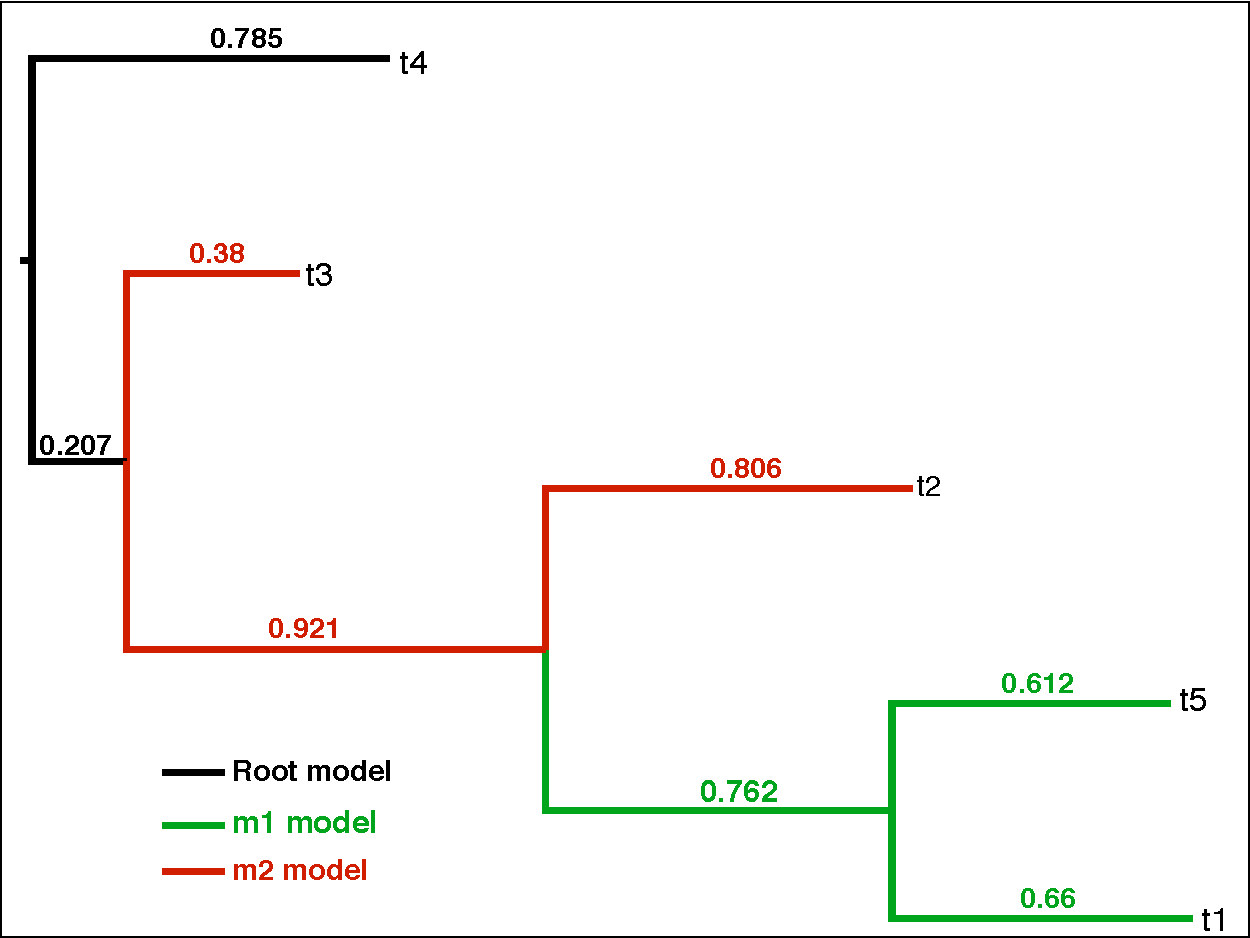
\includegraphics[width=3.75in]{treeflags_colors.pdf}
	\caption{\label{fig:treeflags} The newick tree with model flags given by \\ \texttt{\scriptsize{"(t4:0.785,(t3:0.380,(t2:0.806,(t5:0.612,t1:0.660):0.762\_m1\_):0.921\_m2\_):0.207);"}}
		indicates the model assignments shown.}
\end{figure}


All model flags specified in the newick phylogeny must have corresponding models. To link a model to a model flag, specify a given model's name using the keyword argument \code{name} when initializing a \code{Model} object. This name must be identical to a given model flag, \emph{without} the leading and trailing underscores (e.g.\ the name "m1" corresponds to the flag \_m1\_).

The model at the root of the tree will not have a specific model flag, but nonetheless a model must be used at the root (obviously), and indeed at all other nodes which are not assigned a model flag (not that all branches on the tree which are not assigned a model flag will evolve according to the model used at the root). To specify a model at the root of the tree, simply create a model, with a name, and indicate this name when defining your partition.

Examples for defining models with names are shown below (for demonstrative purposes, nucleotide models with extreme state frequency differences are used here):
\begin{lstlisting}
# Define the m1 model, with frequencies skewed for AT-bias
m1_model = pyvolve.Model("nucleotide", {"state_freqs":[0.4, 0.1, 0.1, 0.4]}, name = "m1")

# Define the m2 model, with frequencies skewed for GC-bias
m2_model = pyvolve.Model("nucleotide", {"state_freqs":[0.1, 0.4, 0.4, 0.1]}, name = "m2")

# Define the root model, with default equal nucleotide frequecies
root_model = pyvolve.Model("nucleotide", name = "root")
\end{lstlisting}

Alternatively, you can assign/re-assign a model's name with the \code{.assign\_name()} method:
\begin{lstlisting}
# (Re-)assign the name of the root model
root_model.assign_name("new_root_model_name")
\end{lstlisting}



Finally, when defining the partition that uses all of these models, provide all \code{Model} objects in list to the \code{models} argument. In addition, you \emph{must} specify the name of the model you wish to use at the root of the tree with the keyword argument \code{root\_model\_name}.
\begin{lstlisting}
# Define partition with branch heterogeneity, with 50 nucleotide positions
temp_het_partition = pyvolve.Partition(models = [m1_model, m2_model, root_model], size = 50, root_model_name = root_model.name) 
\end{lstlisting}



\section{Implementing branch-site heterogeneity}

Simulating according to so-called "branch-site" models, in which there are both site-wise and branch heterogeneity, is accomplished using the same strategies shown for each individual aspect (branch, Section~\ref{sec:branchhet} and site, Section~\ref{sec:sitehet}). However, there is a critical caveat to these models: all models within a given partition \emph{must} have the same number of rate categories. Furthermore, the rate probabilities must be the same across models within a partition; if different values for \code{rate\_probs} are indicated, then the probabilities provided for the \emph{root model} will be applied to all subsequent branch models. (Note that this behavior is identical for other simulation platforms, like Indelible \citep{Fletcher2009}.)

The example below shows how to specify a branch-site heterogeneous nucleotide model with two models, root and model1 (note that this code assumes that the provided phylogeny contained the flag \code{\_model1\_}), when the rate categories are \emph{not} equiprobable.
\begin{lstlisting}
# Shared rate probabilities. Must be explicitly specified for all models (not just the root model)!
shared_rate_probs = [0.25, 0.3, 0.45]

# Construct a nucleotide model with 3 rate categories
root = Model("nucleotide", name = "root", rate_probs = shared_rate_probs, rate_factors = [1.5, 1.0, 0.05])

# Construct a second nucleotide model with 3 rate categories
model1 = Model("nucleotide", name = "model1", rate_probs = shared_rate_probs, rate_factors = [0.06, 2.5, 0.11])

# Construct a partition with these models, defining the root model nameas "root"
part = Partition(models = [root, model1], root_model_name = "root", size = 50)
\end{lstlisting}





\section{Special Pyvolve Features}\label{sec:special}

This section details special features in to Pyvolve, relative to other sequence simulation platforms.

\subsection{Specifying custom rate matrices}\label{sec:custom}

Rather than using a built-in modeling framework, you can specify a custom rate matrix. This rate matrix must be square and all rows in this matrix must sum to 0. Pyvolve will perform limited sanity checks on your matrix to ensure that these conditions are met, but beyond this, Pyvolve takes your matrix at face-value. In particular, Pyvolve will not scale the matrix in any manner. Note that Pyvolve will automatically determine the equilibrium frequencies from your provided matrix, and any frequencies you provide will be overwritten. 

When providing a custom matrix, you also have the option to provide a custom \emph{code}, or custom states which are evolved. In this way, you can evolve characters of any kind according to any specified transition matrix. If you do not provide a custom code, Pyvolve checks to make sure that your matrix has dimensions of either $4\times4$, $20\times20$, or $61\times61$ (for nucleotide, amino-acid, or codon evolution, respectively). Otherwise, Pyvolve will check that your provided code and matrix are compatible (in terms of dimensions). Providing a custom code is, therefore, an attractive option for specifying arbitrary models of character evolution.

To specify a custom rate matrix, provide the argument \code{"custom"} as the first argument when defining a \code{Model} object, and provide your matrix in the custom-parameters dictionary using the key \code{matrix}. Any custom matrix specified should be either a 2D numpy array or a python list of lists. Below is an example of specifying a custom nucleotide rate matrix:
\begin{lstlisting}
import numpy as np # import to construct matrix

# Define a 4x4 custom rate matrix
custom_matrix= np.array([[-1.0, 0.33, 0.33, 0.34], 
                         [0.25, -1.0, 0.25, 0.50], 
                         [0.10, 0.80, -1.0, 0.10],
                         [0.34, 0.33, 0.33, -1.0]] )

# Construct a model using the custom rate-matrix
custom_model = pyvolve.Model("custom", {"matrix":custom_matrix})
\end{lstlisting}
Pyvolve automatically assumes that any $4\times4$ matrix indicates nucleotide evolution. As stated above, Pyvolve will extract equilibrium frequencies from this matrix and check that they are acceptable. This frequency vector will be automatically saved to a file called "custom\_matrix\_frequencies.txt", and these values will be used to generate the root sequence during simulation.

To provide a custom code, include the additional key \code{"code"}in your dictionary. Note that this key would be ignored for any built-in model.
\begin{lstlisting}
import numpy as np # import to construct matrix

# Define a 3x3 custom rate matrix
custom_matrix= np.array([[-0.50, 0.30, 0.20], 
					     [0.25, -0.50, 0.25], 
                         [0.40, 0.10, 0.50]] )

custom_code = ["0", "1", "2"]
# Construct a model using the custom rate-matrix and the custom code
custom_model = pyvolve.Model("custom", {"matrix":custom_matrix, "code":custom_code})
\end{lstlisting}

The resulting data simulated using the above model will contain characters 0, 1, and 2. Although the above example shows a $3\times3$ matrix, it is certainly possible to specify custom matrices and codes for the "standard" dimensions of 4, 20, and 61. 





\subsection{Matrix scaling options}\label{sec:scaling}

By convention, rate matrices are scaled such that the mean substitution rate is 1:
\begin{equation}\label{eq:scaling}
- \sum_{i=1} \pi_iq_{ii} = 1
\end{equation}
\citep{GY94,Yang1994}. Using this regime, branch lengths explicitly indicate the expected number of substitutions per unit (nucleotide, amino acid, or codon). By default, Pyvolve will scale rate matrices according to equation~\ref{eq:scaling}, as this approach remains conventional in the field. 

Unfortunately, this scaling approach can lead to some unexpected results for modeling frameworks which contain explicit parameters for natural selection (mechanistic codon and MutSel models). For example, when multiple mechanistic codon ($dN/dS$) models are used, thus allowing for variable $dN/dS$ values across sites, multiple rate matrices must be used -- one matrix per $dN/dS$ value. This scaling approach, then, would cause sites with $dN/dS = 0.05$ to experience the same average number of substitutions as sites with $dN/dS = 2.5$. From a biological perspective, this result is undesirable, as sites with low $dN/dS$ values should evolve more slowly than sites with high $dN/dS$ values. Figure~\ref{fig:yang_vs_neutral} demonstrates the distinction between the conventional scaling approach [equation ~\eqref{eq:scaling}], which we call "Yang", and our neutral scaling approach.

\begin{figure}[h]
	\centerline{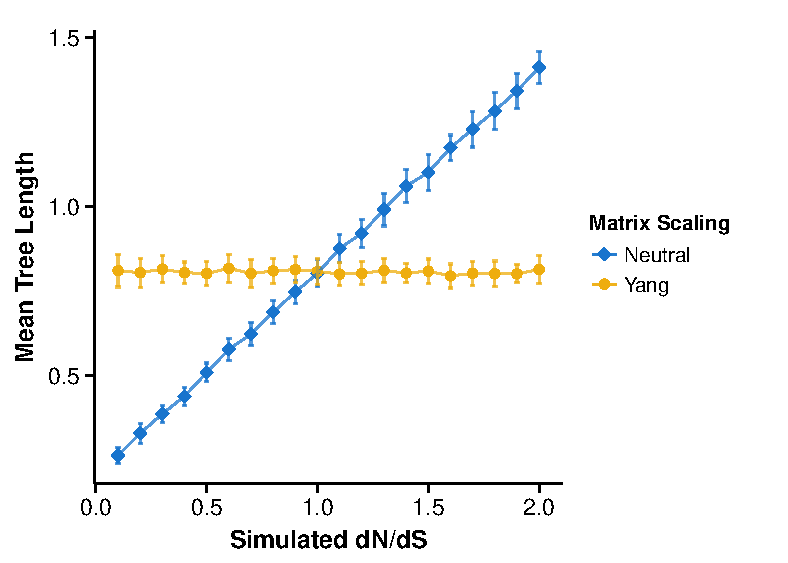
\includegraphics[width=3in]{yang_neutral_scaling.pdf}}
	\caption{\footnotesize{Neutral scaling approach yields more realistic simulations than the Yang (equation \eqref{eq:scaling}) approach. Using Pyvolve, we simulated alignments, of 200 codons each, under the GY94 \citep{GY94,NielsenYang1998} mechanistic codon model. All simulations were performed along the same, randomly generated (using the rtree function in the R package APE \citep{ape}) 25-taxon tree. We simulated alignments (50 replicates each) with a global $dN/dS$ value ranging from 0.1 - 2.0, for each scaling approach. For each resulting alignment, we inferred a maximum-likelihood phylogeny with RAxML \citep{raxml} under the GTRGAMMA model. We then used DendroPy \citep{dendropy} to calculate a tree length for each inferred phylogeny, indicating the average number of substitutions in the full tree. This figure demonstrates that the average number of substitutions remains constant across $dN/dS$ values when the Yang scaling approach is applied, but this value increases linearly when Pyvolve's neutral scaling approach is applied. Further, the Yang and neutral scaling approaches yield the same number of average substitutions when $dN/dS = 1$, as expected. Error bars represent standard deviations.}}\label{fig:yang_vs_neutral}
\end{figure}


To overcome this issue, Pyvolve provides an option to scale matrices such that the mean \textit{neutral} substitution rate is 1. For $dN/dS$ codon models, this approach scales the matrix such that the mean number of substitutions when $dN/dS = 1$ is 1. For mutation-selection models (both nucleotide and codon), this approach scales the matrix such that the mean substitution rate is 1 when all states (nucleotides/codons) have equal fitness. Note that invoking neutral-scaling option has no effect on nucleotide or amino-acid models!

To invoke the neutral scaling, provide the keyword argument \code{scale\_matrix = "neutral"} argument "neutral" when defining a Model object:
\begin{lstlisting}
# Construct a codon model with neutral-scaling
m = pyvolve.Model("GY94", {"omega":0.5}, scale_matrix = "neutral") 
\end{lstlisting}

While we believe that this neutral scaling approach leads to more realistic simulated data, we urge caution when using this scaling approach. Most phylogenetic inference softwares and modeling frameworks (including HyPhy \citep{HYPHY} and PAML \citep{PAML}), scale matrices according to equation~\ref{eq:scaling}, and thus inferences on data simulated with neutral scaling may be confounded due to conventions in third-party softwares.


\subsection{Perturbing branch lengths}\label{sec:noisybl}

Conventional sequence simulation algorithms apply a given branch length uniformly across a given branch. For example, if a given branch has a length of 0.1, then every site along that branch will evolve with a branch length of exactly 0.1. However, given that phylogenetic inference methods compute branch lengths effectively as an average value for all sites along that branch, there is no reasonable justification to assume all sites should have an identical branch length.

Therefore, Pyvolve allows you to specify some amount of noise in the branch lengths. Specifically, you can opt to draw \emph{site-specific} branch lengths from one of three distributions: normal, gamma, or exponential. Each scheme will retain the given branch length in the newick phylogeny as the average branch length across sites. Given a distribution, Pyvolve will sample, at each branch, a certain number of new branch lengths (default is 10\% of the sequence length) and apply these randomly to each evolving site. 

To invoke perturbed branch lengths, use the keyword argument \code{branch\_lengths} when \emph{defining} (not calling!) an \code{Evolver} object. This argument should be a \emph{dictionary} with keys indicating the distribution and any distribution-specific parameters. The distribution should be specified with the key \code{"dist"} as either "normal", "gamma", or "exp" (for exponential). Normal distributions require the additional key \code{"sd"} for standard deviation, and gamma distributions require the additional key of either \code{"shape"} or \code{"alpha"} (treated equivalently) to specify the shape. Exponential distributions require no other keys.


\begin{lstlisting}
# Specify perturbed branch lengths according to different distributions

# Normal distribution with a standard deviation of 0.1
my_evolver = Evolver(partitions = my_partitions, tree = my_tree, branch_lengths = {"dist":"normal", "sd":0.1})

# Gamma distribution with a shape of 0.5
my_evolver = Evolver(partitions = my_partitions, tree = my_tree, branch_lengths = {"dist":"gamma", "shape":0.5}) # can use "alpha" key instead of "shape", if desired

# Exponential distribution
my_evolver = Evolver(partitions = my_partitions, tree = my_tree, branch_lengths = {"dist":"exp"})
\end{lstlisting}

Finally, you can change the number of site-wise branch lengths, for each branch, to sample with the key \code{"num\_categories"}. Specify a number in the range 1 - sequence length, or alternatively to specify a completely unique branch length at every site, you can set the value as "full". (Remember - the default number of branch lengths to draw is 10\% of the sequence length).

\begin{lstlisting}
# Specify 20 branch length categories per branch (uses exponential distribution as example)
my_evolver = Evolver(partitions = my_partitions, tree = my_tree, branch_lengths = {"dist":"exp", "num_categories": 20})
 
# Specify that every site should have a unique branch length at every branch
my_evolver = Evolver(partitions = my_partitions, tree = my_tree, branch_lengths = {"dist":"exp", "num_categories": "full"})
\end{lstlisting}


%\section{Insertions and Deletions}
%
%At this time, Pyvolve does not support insertions and deletions ("indels"). The main reason for this is that there is currently no obvious way to specify the evolution of inserted sequences. Standard simulation approaches will evolve inserted sequences like any other region: the inserted sequence will be drawn from a specified equilibrium frequency distribution, and then the inserted region will evolve according to a specified rate matrix. Typically, these parameters are taken directly from the model used in the insertion region. This setup is not, however, ideal... 


%\noindent This is my first python example:
%\pythonexternal{script.py}












\bibliographystyle{plain}
\bibliography{citations}





\end{document}